\newpage
\section{Conservation Laws}

Recall how we mentioned heat is conserved, accumulated heat is heat in - heat our.

1-D Conservation:
\begin{itemize}
  \item $u(x, t)$: Quantity that is conserved: energy, mass, momentum, $\ldots$.
\end{itemize}
  %o======|##|======o <- |x0   |x1
  %
  \begin{align}
    g(x, t) & = \text{ flux} = f(u(x, t))
  \end{align}

  Here, flux is dependent on the gradient. Before, we have:
  %
  \begin{align}
    g(x, t) & = g(u_x(x, t))
  \end{align}
  This was our gradient.

  \topic{Conservation Law}

  \begin{center}
    Accumulation = in - out
  \end{center}
  \begin{align}
    \int^{x_1}_{x_0} u(x, t_1) \text dx - \int^{x_1}_{x_0} u(x, t_0) \text dx
    & = u(x_0, t)\\
    \int^x_{x_0} [u(x, t_1) - u(x, t_0)] \text dx
    & = \int^{t_1}_{t_0} [ q(x_0, t) - q(x_1, t)] \text dt\\
    \int^{x_1}_{x_0} \int^{t_1}_{t_0} q_t(x, t) \text dt\ \text dx
    & = - \int^{t_1}_{t_0} \int^{x_1}_{x_0} q_x(x, t) \text dx\ \text dt\\
    \int^{t_1}_{t_0} \int^{x_1}_{x_0} [u_t(x, t) + u_x(x, t)] \text dx\ \text dt
    & = -\int^{t_1}_{t_0} \int^{x_1}_{x_0} q_x(x, t) \text dx\ \text dt\\
    \int^{t_1}_{t_0} \int^{x_1}_{x_0} [u_t(x, t) + q_x(x, t)] \text dx\ \text dt & = 0
  \end{align}

  Here, $u_t + q_x = 0$ if $u_t$ and $q_x$ are continuous.

  Since $q = f(u)$, we get
  %
  \begin{align}
    u_t + [f(u)]_x & = 0
  \end{align}

  This is considered the conservation law. This is non-linear, first order.

  \ex Burger's Equation: For gas flow down a pipe.
  %
  \begin{align}
    u_t + \left( \frac{u^2}{2} \right)_x & = \eps u_{xx}
  \end{align}

  Here, $\eps$ is the viscosity and $u$ is the momentum. The viscosity of gases tend towards zero, therefore let us consider $\eps = 0$.
  %
  \begin{align}
    u_t + \left( \frac{u^2}{2} \right)_x & = 0
  \end{align}
  Here, let $f(u) = \frac{u^2}{2}$:
  \begin{align}
    u_t + u u_x & = 0
  \end{align}

  Domain: $x \in (-\infty, \infty), t \in [0, \infty)$
  % If we have any t partials, we need one initial condition.

  Initial condition: $u(x, 0) = g(x)$

  \underline{Recall}: Transport equation:

  $u_t = cu_x \Rightarrow u_t - cu_x = 0$

  $u(x, 0) = g(x)$.

  The slope of the characteristic $ = -\frac{1}{c}$
  % Graph with $-\frac{1}{c} + k, Vk

  The values of the solution is constant along characteristic.

  \topic{March 30, 2022}

  \subsection{Burger's Equation}
  %
  \begin{align}
    u_t + uu_x & = 0
  \end{align}

  The slope is $\frac{1}{u}$.

  Recall, the slope of the characteristic of the equation $u_t - cu_x = 0$ is $-\frac{1}{c}$.

  \ex
  %
  \begin{align}
    u(x, 0) & =
    \begin{cases}
      1     &         x < 0\\
      1 - x & 0 \leq  x < 1\\
      0     & x \geq  1
    \end{cases}
  \end{align}

  % Graph, ////. /^ /^^ /^^^ . ||||||||

  At $t = 1$, the solution is no longer continuous, therefore $u_x$ is not defined at $x = 1, t = 1$.

  For $t \geq 1$, there is no differentiable solution (everywhere).

  % Slope 1 continues until hitting \infty slope

  If we allow solutions that aren't defined only for a single curve $\xi(t)$ of discontinuity, then we have an infinite number of solutions. From physics, we know that gas velocity (momentum) looks like this:

  % From x = t = 1, Slope 2 appears

  The shock in velocity causes a sonic boom
  %
  \begin{align}
    \text{Slope } & = 2\\
    \xi^\prime(t) & = \frac{1}{2}
  \end{align}
  %
  $u_t + [f(u)]_x = 0$ has no classical solution (existence problem) and $\infty$ number of solutions if we don't care about the equation being satisfied on shocks (uniqueness problem)

  We would like:
  %
  \begin{enumerate}
    \item a unique solution to exist
    \item We want this solution to be what we observe
  \end{enumerate}

  Define a weak solution to be $u(x, t)$ where
  %
  \begin{align}
    \int^{t_1}_{t_0} \int^{x_1}_{x_0} [u_t + [f(u)]_x] \text dx \text dt & = 0
  \end{align}

  where $u_t$ and $[f(u)]_x$ are measures (they can contain $\delta$ functions)

  This idea will lead to a formula for shock speed, $\xi^\prime(t)$.

  The integral in $x-$direction is enough.
  %
  \begin{align}
    \int^{x_1}_{x_0} [u_t + [f(u)]_x]\ \text dx|_{t = t_0} & = 0
  \end{align}

  Here,
  %
  \begin{align}
    \int^{x_1}_{x_0} u_t\ \text dx
    & = - \int^{x_1}_{x_0} [f(u)]_x\ \text dx |_{t = t_0}\\
    \frac{d}{dt} \int^{x_1}_{x_0} u\ \text dx |_{t = t_0}
    & = f(u(x_0, t_0) - f(u(x_1, t_0)))\\
    \frac{d}{dt} \left[ \int^{\xi(t)}_{x_0} u(x, t)\ \text dx + \int^{x_1}_{\xi(t)} u(x, t)\ \text dx \right] \big|_{t = t_0}
    & = f(u_L) - f(u_R)
  \end{align}

  Using the second fundamental theorem of calculus,
  %
  \begin{align}
    \int^{\xi(t)}_{x_0} u_t(x, t) \text dx + u(\xi(t), t) \xi^\prime(t) + \int^{x_1}_{\xi(t)} u_t(x, t) \text dx - u(\xi(t), t)\xi^\prime(t)|_{t = t_0} & = f(u_L) - f(u_R)
  \end{align}

  You cannot cancel the second and fourth term, as the second term is on the left of the shock and the fourth term is on the right of the shock.

  Take $\lim$ as $x_0 \to \xi(t)^-$,
  %
  \begin{align}
    \int^{\xi(t)}_{x_0} u_t(x, t) \text dx & = 0
  \end{align}

  Take $\lim$ as $x_1 \to \xi(t)^+$,
  %
  \begin{align}
    \int^{x_1} u_t(x, t) \text dx & = 0
  \end{align}

  We now have:
  %
  \begin{align}
    u_L \xi^\prime(t_0) - u_R \xi^\prime(t_0) & = f(u_L) - f(u_R)
  \end{align}

  $t_0$ is arbitrary.
  %
  \begin{align}
    \xi^\prime(t) & = \frac{f(u_L) - f(u_R)}{u_L - u_R}
  \end{align}

  Here, we have Rankine-Hugniot jump condition.

  \topic{April 1, 2022}
  %
  \begin{align}
    \xi^\prime(t) & = \frac{f(u_L) - f(u_R)}{u_L - u_R}
  \end{align}

  For some example $f(u) = \frac{u^2}{2}$, $u_L = 1, u_R = 0$
  %
  \begin{align}
    \xi^\prime(t) & = \frac{\frac{1}{2} - 0}{1 - 0}\\
    & = \frac{1}{2}
  \end{align}

  There are other initial conditions that still lead to two solutions.
  %
  \begin{align}
    u_t + uu_x & = 0\\
    u(x, 0) & =
    \begin{cases}
      0 & x < 0\\
      1 & e \geq 0
    \end{cases}
  \end{align}

  Riemann Problem. The slope of our characteristic line is $\frac{1}{u}$.

  In our solution, we have the verticals on the left side and slope = 1 on the right side, so the solutions do not collide. To remediate this, we add a shock in between and extend both solutions to the shock line.

  R-H Jump Condition
  %
  \begin{align}
    \xi^\prime(t) & = \frac{0 - \frac{1}{2}}{0 - 1}\\
    & = \frac{1}{2}
  \end{align}

  Another solution is to make a fan (paper fan)

  There would be no shock and the solution is continuous. The R-H jump condition is not used.
  %
  \begin{align}
    u(x, t) & =
    \begin{cases}
      0 & x < 0\\
      \frac{x}{t} & 0 \frac{x}{t} < 1\\
      1 & \frac{x}{t} \geq 1
    \end{cases}
  \end{align}

  Conservation Law: $u_t + [f(u)]_x = 0$.

  If $f$ is smooth: $u_t + f^\prime(u) u_x = 0$.

  $f^\prime(u)$ is the speed of the characteristic.

  Slope of characteristic $= \frac{1}{f^\prime(u)}$

  \note If the solution is continuous, the $R-H$ condition gives the slope of a characteristic, not the slope of shocks.

  What is the actual solution to the last problem?
  %
  \begin{align}
    u_t + u u_x & = \eps u_{xx}
  \end{align}

  Therefore, if $\eps > 0$ is a smoothing term (as in heat) $\to C^\infty$.

  Which solution is the solution that you get if you solve the last equation and let $\eps \to 0$?

  This ends up giving us the lax entropy condition:

  The characteristic curves can enter a shock as time increases, but they cannot exit (or be created) from a shock.

  % Solution one: tree leaf, branch out from center stem
  % Solution two: hut
  Solution one violates the lax entropy condition, therefore solution two is the correct solution.

  \thm There exists a unique solution to any conservation law $u_t + [f(u)]_x = 0$, $u(x, 0) = g(x)$, $x \in (-\infty, \infty), t \in [0, \infty)$ whose shocks satisfy the $R-H$ jump condition and the lax entropy condition.

  \note The fan is called a carefaction wave.

  For any general first order equation $F(\vv x, u(\vv x), \grad(\vv x)) = 0$

  $\vv x = (x, t)$ is our conservation law, you always have characteristic curves. The difficulty lies with how to resolve what happens when characteristic collide.

  \subsection{Traffic Flow}
  \topic{April 11, 2022}
  Conservation of Cars

  Traffic in - Traffic out = Accumulated traffic

  \begin{center}
    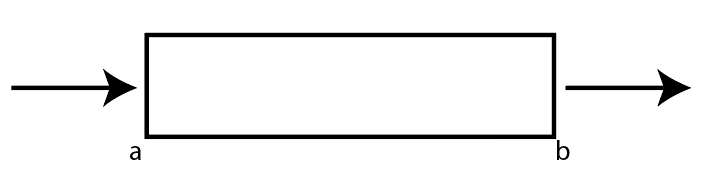
\includegraphics{Conservation Laws - Traffic Flow 1}
  \end{center}

  Let $\rho(x, t)$ be the density and $q(x, t)$ is the flux.
  %
  \begin{align}
    \frac{d}{dt} \int^b_a \rho(x, t)\ \text dx
    & = q(a, t) - q(b, t)\\
    & = -\int^b_a q_x (x, t)\ \text dx\\
    \int^b_a (\rho_t + q_x)\ \text dx & = 0\\
    \rho_t + q_x & = 0
  \end{align}

  Here, $u$ is car velocity:
  %
  \begin{align}
    q & = pu
  \end{align}

  Now,
  %
  \begin{align}
    \rho_t + [\rho u]_x & = 0
  \end{align}

  Both $\rho$ and $u$ are a function of $x$, therefore there is a
  product rule that comes into play.
  %
  \begin{align}
    \rho_t + [c(\rho)]\rho_x & = 0
  \end{align}

  We have yet to determine $c$. So far, this equation is similar to the Transport
  Equation, where we use $c$ to find the speed of the equation.

  $c(\rho)$ will give the speed of the characteristic.

  In general, the car velocity should be a decreasing function of $\rho$.

  When $\rho = 0$, the car moves the fastest $= u_{\text{max}}$

  When $\rho = \rho_{\text{max}} \Rightarrow u = 0$

  The simplest relationship which satisfies these is:
  %
  \begin{align}
    u(\rho) & = u_{\text{max}}\left(1 - \frac{\rho}{\rho_{\text{max}}}\right)
  \end{align}

  This tells me,
  %
  \begin{align}
    q(\rho)
    & = u_{\text{max}} \rho\left( 1 - \frac{\rho}{\rho_{\text{max}}}\right)\\
    & = u_{\text{max}} \rho - \frac{u_{\text{max}}}{\rho_{\text{max}}} \rho^2
  \end{align}

  Hit maximum velocity at $\frac{\rho_{text{max}}}{2}$
  %
  \begin{align}
    q_x
    & = u_{\text{max}} \rho_x - 2 \frac{u_{\max}}{\rho_{\max}} \rho \rho_x\\
    & = u_{\max} \left[ 1 - \frac{2}{\rho_{\max}} \rho \right] \rho_x
  \end{align}

  Here, this shows our critical point is at $\frac{\rho_{\max}}{2}$. Let us
  redefine this equation as $c(\rho) \rho_x$.
  %
  \begin{align}
    \rho_t + u_{\max} \left( 1 - \frac{2\rho}{\rho_{\max}}\right) \rho_x & = 0
  \end{align}

  \ex When a red light turns green.
  %
  \begin{align}
    \rho(x, t) & =
    \begin{cases}
      \rho_{\max} & x < 0\\
      0 & x > 0
    \end{cases}
  \end{align}

  Recall, the speed of our characteristic:
  %
  \begin{align}
    c(\rho) & = u_{\max} \left(1 - \frac{2 \rho}{\rho_{\max}}\right)
  \end{align}

  The slope of our characteristic is:
  %
  \begin{align}
    & = \frac{1}{u_{\max} \left(1 - \frac{2 \rho}{\rho_{\max}}\right)}
  \end{align}

  When we have $\rho = \rho_{\max}$, our slope is $- \frac{1}{u_{\max}}$.

  When we have $\rho = 0$, our slope is $\frac{1}{u_{\max}}$.
  %
  \begin{align}
    \rho(x, t) & =
    \begin{cases}
      \rho_{\max} & x < - u_{\max} t\\
      \frac{\rho_{\max}}{2} \left(1 - \frac{x}{u_{\max}t}\right)
      & -u_{\max} t < x < u_{\max} t\\
      0 & x > u_{\max} t
    \end{cases}
  \end{align}

  \ex When the light turns red, hit bumper-to-bumper traffic.

  For $x < 0$, we have $\rho(x, 0) = \rho_0$.

  For $x > 0$, we have $\rho(x, 0) = \rho_{\max}$.

  Here, let us write:
  %
  \begin{align}
    u_t + [f(u)]_x & = 0\\
    \xi^\prime(\aleph) & = \frac{f(u_L) - f(u_R)}{u_L - u_R}
  \end{align}

  Our $q$ is:
  %
  \begin{align}
    q(\rho) = u_{\max} \rho\left(1 - \frac{\rho}{\rho_{\max}}\right)
  \end{align}

  If we consider our graph, a shock will form and we will have:
  %
  \begin{align}
    \xi^\prime(t) & = \frac{q(\rho_L) - q(\rho_R)}{\rho_L - \rho_R}\\
    & = \frac{u_{\max} \rho_0 \left( 1 - \frac{\rho_0}{\rho_{\max}
    - 0}\right)}{\rho_0 - \rho_{\max}} < 0
  \end{align}

  \topic{April 13, 2022}

  \ex Green light turns red, then green

  \begin{center}
    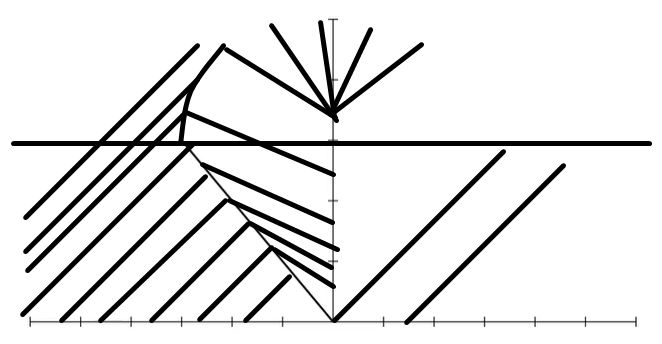
\includegraphics{Traffic Light - Turning Red}
  \end{center}

  \subsection{Method of Characteristics}

  We will look at agns? of the form:
  %
  \begin{align}
    a(x, t) u_x + b(x, t) u_t + c(x, t) u & = 0\\
    u(x, 0) & = f(x)
  \end{align}

  Let:
  %
  \begin{itemize}
    \item $x(t)$ : Moving observer <- Location of observer
    \item $u(x, t)$ : function of $x$ and $t$
  \end{itemize}

  How does $u$ change from the observer's perspective?

  How does a point in front of one move?

  Find $\frac{du}{dt}$:
  %
  \begin{align}
    \frac{du(x(t), t)}{dt} & = \frac{du}{dt} + \frac{\p u}{\p x} \frac{dx}{dt}\\
    & = u_t + u_x \frac{dx}{dt}
  \end{align}

  \ex Transport Equation
  %
  \begin{align}
    u_t + cu_x & = 0\\
    \frac{dx}{dt} & = c\\
    \frac{du}{dt} & = 0
  \end{align}

  The observer is moving at speed $c$ and $u$ is not changing.

  Let us consider the following:
  %
  \begin{align}
    u(x, 0) & = f(x)\\
    x(0) & = x_0\\
    u(0) & = u_0
  \end{align}

  Now, let us consider:
  %
  \begin{align}
    \frac{du}{dt} & = u_t + \frac{dx}{dt} u_x
  \end{align}
  \begin{align}
    \frac{dx}{dt} & = c\\
    x & = ct + k\\
    x & = ct + x_0\\
  \end{align}
  \begin{align}
    \frac{du}{dt} & = 0\\
    u & = u_0\\ & = u(x_0, 0)\\ & = f(x_0)\\ & = f(x - ct)
  \end{align}

  \note
  %
  \begin{align}
    u_t + cu_x & = 0\\
    \left< 1, c \right> \cdot \left< u_t, u_x \right> & = 0\\
    \left< 1, c \right> \cdot \left< \grad \right> & = 0
  \end{align}

  Here, we found the directional derivative.

  \ex $u_t + cu_x = 1$ and $u(x, 0) = \sin x$
  %
  \begin{align}
    \frac{dx}{dt} = c & \Rightarrow x = ct + x_0\\
    \frac{du}{dt} = 1 & \Rightarrow u = t + B\\
    u(x_0, t) & = u_0\\
    & = t + u_0 = t + u(x_0, 0)\\
    & = t + \sin x_0\\
    & = t + \sin(x - ct)
  \end{align}

  \ex $u_t + cu_x + au = 0$, $u(x, 0) = f(x)$
  %
  \begin{align}
    u_t + cu_x & = -au\\
    \left< 1, c \right> \cdot \left< u_t, u_x \right> & = -au
  \end{align}

  If $a > 0$, directional derivative $= -au \Rightarrow$ decay
  %
  \begin{align}
    \frac{dx}{dt} = c & \Rightarrow x = ct + x_0
  \end{align}

  The following is an exponential decay (Refer to Differential Equation):
  %
  \begin{align}
    \frac{du}{dt} & = -au\\
    u & = De^{-at} = u_0 e^{-at}
  \end{align}

  When we plug in $t = 0$, we should get $f(x)$:
  %
  \begin{align}
    u & = f(x_0) e^{-at}\\
    & = f(x - ct) e^{-at}
  \end{align}

  \ex $u_t + xu_x = 0$, $u(x, 0) = f(x)$
  %
  \begin{align}
    \frac{dx}{dt} = x & \Rightarrow x = x_0 e^t\\
    \frac{du}{dt} = 0 & \Rightarrow u = u_0 = f(x_0) = \left(\frac{x}{e^t}\right)
    = f(xe^{-t})
  \end{align}

  \topic{April 18, 2022}
  %
  \begin{align}
    \frac{du}{dt} & = \frac{dx}{dt} u_x + u_t
  \end{align}

  We can also introduce a new variable,
  %
  \begin{align}
    a(x, t) u_x + b(x, t) u_t + c(x, t) u & = 0\\
    \frac{dx}{ds} & = a(x, t)
  \end{align}

  \begin{multicols}{2}
    \begin{align}
      \frac{dx}{ds} & = a(x, t)\\
      \frac{dt}{ds} & = b(x, t)
    \end{align}

    \begin{align}
      \frac{dy}{ds} & = -c(x, t) u\\
      \frac{du}{ds} & = \frac{dx}{ds} u_x + \frac{dt}{ds} u_t
    \end{align}
  \end{multicols}

  \begin{center}
    \import{Snippets/}{tree_uxts}
  \end{center}

  \ex $xu_x + u_t + tu = 0 \Rightarrow xu_x + u_t = -tu$
  %
  \begin{align}
    \frac{dx}{ds} & = x \Rightarrow x = ce^s = x_0 e^s = x_0 e^t\\
    \frac{dt}{ds} & = 1 \Rightarrow t = s + t_0 = s\\
    \frac{du}{ds} & = -tu = -su \Rightarrow u = f\left(xe^{-t}\right)
    e^{-\frac{1}{2}t^2}
  \end{align}

  To find the third differential, we did separation of variables:
  %
  \begin{align}
    \int \frac{1}{u} du & = \int -s ds\\
    \ln |u| & = - \frac{1}{2} s^2 + c\\
    u & = e^{- \frac{1}{2} s^2 + c}\\
    u & = ce^{- \frac{1}{2} s^2}\\
    u & = u_0 e^{-\frac{1}{2} t^2}\\
    u & = f(x_0) e^{-\frac{1}{2}t^2}\\
    u & = f\left(xe^{-t}\right)e^{-\frac{1}{2}t^2}
  \end{align}

  Because $u(x 0) = f(x)$ and $x_0 = \frac{x}{e^t} = xe^{-t}$

  \ex $2xtu_x + u_t = u$, $u(x, 0) = x$

  Because $\frac{dt}{ds} = 1$, we do not consider $s$.
  %
  \begin{align}
    \frac{dx}{dt} & = 2xt \Rightarrow x = x_0 e^{t^2}\\
    \frac{du}{dt} & = u \Rightarrow u = u_0 e^t = f(x_0) e^t = f(xe^{-t^2})e^t
    = xe^{-t^2} e^t
  \end{align}

  Recall $u_0 = f(x)$.

  Here, we found $\frac{dx}{dt}$ through separation of variables:
  %
  \begin{align}
    \frac{dx}{dt} & = 2xt\\
    \int \frac{1}{x} & = \int 2t dt\\
    \ln |x| & = t^2 + c\\
    x & = ce^{t^2}\\
    x & = x_0 e^{t^2}
  \end{align}

  \ex $u^2 \frac{du}{dx} + \frac{du}{dt} = 0$, $u(x, 0) = \sqrt x$.
  %
  \begin{align}
    \frac{dx}{dt} & = u^2 \Rightarrow x = u^2 t + c = u^2 t + x_0
    \Rightarrow x_0 = x - u^2 t\\
    \frac{du}{dt} & = 0 \Rightarrow u = u_0 = f(x_0) = f(x - u^2 t)
    = \sqrt{x - u^2 t} = \sqrt{\frac{x}{1 + t}}
  \end{align}

  Here, we solve for $u$ as:
  %
  \begin{align}
    u & = \sqrt{x - u^2 t}\\
    u^2 & = x - u^2 t\\
    u^2(1 + t) & = x\\
    u^2 & = \frac{x}{1 + t}\\
    u & = \sqrt{\frac{x}{1 + t}}
  \end{align}

  \ex $e^{t^2} u_t + tu_x = 0$, $u(x, 0) = f(x)$.

  Here, let us divide out our term in front of
  $u_t$ to get $u_t + te^{-t^2}u_x = 0$,
  %
  \begin{align}
    \frac{dx}{dt} & = te^{-t^2} \Rightarrow x = \\
    \frac{du}{dt} & = 0 \Rightarrow u = u_0 = f(x_0)
    = f(x + \frac{1}{2}e^{-t^2} - \frac{1}{2})
  \end{align}

  To solve for $x$,
  %
  \begin{align}
    x & = \int te^{-t^2}\\
    & = -\frac{1}{2} \int e^w \text dw\\
    & = -\frac{1}{2} e^w + c\\
    & = -\frac{1}{2} e^{-t^2} + C
  \end{align}

  Here, we want our term to zero out:
  %
  \begin{align}
    x_0 & = - \frac{1}{2} + c \Rightarrow c = x_0 + \frac{1}{2}\\
    x & = -\frac{1}{2} e^{t^2} + x_0 + \frac{1}{2}\\
    x_0 & = x + \frac{1}{2} e^{-t^2} - \frac{1}{2}
  \end{align}

  \ex $u_t + tu_x = u^2$, $u(x, 0) = f(x)$
  %
  \begin{align}
    \frac{dx}{dt} & = t \Rightarrow x = \frac{1}{2} t^2 + c
    = \frac{1}{2} t^2 + x_0 \Rightarrow x_0 = x - \frac{1}{2} t^2\\
    \frac{du}{dt} & = u^2 \Rightarrow u =
  \end{align}

  Here, to solve the second term,
  %
  \begin{align}
    \frac{du}{dt} & = u^2\\
    \int \frac{1}{u^2} \text du & = \int \text dt\\
    -\frac{1}{u} & = t + c\\
    \frac{1}{u} & = -t + c\\
    u & = \frac{1}{c - t}\\
    & = \frac{1}{\frac{1}{u_0} - t}\\
    & = \frac{u_0}{1 - u_0 t}\\
    & = \frac{f(x_0)}{1 - f(x_0)t}\\
    & = \frac{f\left(x - \frac{1}{2}t^2\right)}
    {1 - f\left(x - \frac{1}{2}t^2\right)t}
  \end{align}

  \topic{April 20, 2022}

  \ex $tu_x - xu_t = u$ \quad $u(x, 0) = f(x)$
  \begin{align}
    \frac{dx}{ds} & = t\\
    \frac{dt}{ds} & = -x\\
    \frac{du}{ds} & = u
  \end{align}

  Here, the issue with this format is that the first two terms have three
  variables. We must find $x_0$ and to get $x_0$, we must get to $x$. To solve
  this, we will look at parametric equations. Let us combine the first two lines to get:
  %
  \begin{align}
    \frac{dx}{dt} & = - \frac{t}{x}
  \end{align}

  From here, we can solve this via separation of variables
  %
  \begin{align}
    \int x \text dx & = \int - t \text dt\\
    \frac{1}{2} x^2 & = -\frac{1}{2} t^2 + C\\
    x^2 & = - t^2 + C\\
    x^2 + t^2 & = C\\
    x^2 + t^2 & = x^2_0
  \end{align}

  Now, to solve for our third term, we would get an exponential via separation of variables:
  %
  \begin{align}
    \frac{du}{ds} & = u \Rightarrow u = u_0 e^s
  \end{align}

  Here, if we want to find $t$ for $s$, we write:
  %
  \begin{align}
    \frac{dx}{ds} & = t \Rightarrow \frac{d^2x}{ds^2} = \frac{dt}{ds} = -x
    \Rightarrow x(s) = a \cos s + b \sin s\\
    & \Rightarrow x(0) = x_0 \rightarrow a = x_0\\
    \frac{dt}{ds} & = -x \Rightarrow \frac{d^2t}{ds^2} = -\frac{dx}{ds} = -t
    \Rightarrow t(s) = b \cos s - a \sin s\\
    & \Rightarrow t(0) = 0 \rightarrow b = 0
  \end{align}

  Since want to start $t$ at $0$, $\sin$ would belong to $t$.

  Now, we know the following:
  %
  \begin{align}
    x & = x_0 \cos s\\
    t & = -x_0 \sin s\\
    \frac{t}{x} & = - \tan s
  \end{align}

  So, to go back to $\frac{du}{ds}$,
  %
  \begin{align}
    \frac{du}{ds} & = u \Rightarrow u = u_0 e^s
    = f(x_0) e^{\arctan \frac{-t}{x}}\\
    & = f\left( \sqrt{x^2 + t^2} \right) e^{\arctan \frac{-t}{x}}
  \end{align}

  \ex $xu_x + tu_t = 2u$ \quad $u(x_0, 1) = f(x)$
  \begin{align}
    \frac{dx}{ds} & = x \Rightarrow_1 x = x_0 e^s \Rightarrow_4 x_0
    = \frac{x}{e^s} = \frac{x}{t}\\
    \frac{dt}{ds} & = t \Rightarrow_2 t = t_0 e^s = e^s\\
    \frac{du}{ds} & = 2u \Rightarrow_3 u = u_0 e^{2s}
    \Rightarrow_5 u = f(x_0) e^{2s} = f\left(\frac{x}{t}\right)(e^s)^2
    = f\left(\frac{x}{t}\right)t^2
  \end{align}

  \ex $u_t + tu_x = 0$, $u(x, 0) = f(x)$
  %
  \begin{align}
    \frac{dx}{dt} & = t \Rightarrow_1 x = \frac{1}{2}t^2 + x_0\\
    \frac{du}{dt} & = 0 \Rightarrow u = u_0 = f(x_0) = f\left(x - \frac{1}{2} t^2\right)
  \end{align}

  \ex $u_t + tu_x = xt$, $u(x, 0) = f(x)$
  %
  \begin{align}
    \frac{dx}{dt} & = t \Rightarrow_1 x = \frac{1}{2} t^2 + x_0\\
    \frac{du}{dt} & = xt = t\left(\frac{1}{2}t^2 + x_0\right)
    = \frac{1}{2} t^3 + x_0 t\\
    & \Rightarrow_2 u = \frac{1}{8} t^4 + \frac{1}{2} x_0 t^2 + u_0
    = \frac{1}{8} t^4 + \frac{1}{2} \left(x - \frac{1}{2} t^2\right)t^2 +
    f\left(x - \frac{1}{2} t^2 \right)
  \end{align}

  \ex $u_t + xu_x = x$, $u(x, 0) = f(x)$
  %
  \begin{align}
    \frac{dx}{dt} & = x \Rightarrow_1 x_0 e^t\\
    \frac{du}{dt} & = x =_2 x_0e^t \Rightarrow u = x_0e^t + C
    = x_0 e^t + u_0 - x_0 = x + f(xe^{-t}) - xe^{-t}
  \end{align}

  \ex $xu_x + u_t = t$, $u(x, 0) = x^2$
  %
  \begin{align}
    \frac{dx}{dt} & = x \Rightarrow_1 x = x_0 e^t\\
    \frac{du}{dt} & = t \Rightarrow_2 u = \frac{1}{2} t^2 + u_0
    = \frac{1}{2}t^2 + f\left(xe^{-t}\right)
    = \frac{1}{2}t^2 + \left(xe^{-t}\right)^2
  \end{align}

  \ex $xu_t - 2xtu_x = 2tu$, $u(x, 0) = f(x)$

  Let us rewrite our equation as $u_t - 2tu_x = \frac{2tu}{x}$
  %
  \begin{align}
    \frac{dx}{dt} & = -2t \Rightarrow_1 x = -t^2 + x_0\\
    \frac{du}{dt} & = \frac{2tu}{x} =_2 \frac{2tu}{x_0 - t^2}
  \end{align}

  For the second term, we would have to separate:
  %
  \begin{align}
    \int \frac{1}{u} \text du & = \int \frac{2t}{x_0 - t^2} \text dt\\
    \ln |u| & = \int \frac{2t}{x_0 - t^2} \text dt
  \end{align}

  Here, our $w = x_0 t^2$ and $dw = -2t dt$
  %
  \begin{align}
    \ln |u| & = - \ln |x_0 - t^2| + C\\
    u & = ce^{-\ln|x_0 - t^2|}\\
    u & = ce^{\ln|x_0 - t^2|^{-1}}\\
    u & = \frac{c}{x_0 - t^2}
  \end{align}

  Here, we know $x_0$ and we can find $c$ since plugging in $0$ should give us
  $u_0$:
  %
  \begin{align}
    & = \frac{x_0 u_0}{x_0 - t^2}\\
    u & = \frac{(x + t^2) f(x_0 + t^2)}{x}
  \end{align}
